\section{Simulation studies}\label{section:Simulations}

We conduct two sets of simulation studies to evaluate the empirical performance of the proposed Causal Horseshoe Forest. 
The first set assesses general accuracy and uncertainty quantification for estimating heterogeneous treatment effects under varying levels of dimensionality.
The second set focuses on a more targeted scenario designed to study regularisation-induced confounding.

\subsection{General performance}\label{sec:sim-setup}

We compare the Causal Horseshoe Forest to several AFT-based Bayesian tree ensemble methods commonly used for heterogeneous treatment effect estimation.
We consider the following models:
{\setlength{\itemsep}{1pt}
 \setlength{\parsep}{0pt}
\begin{itemize}
    \item \textbf{Causal Horseshoe Forest}: our proposed method, with shrinkage parameter $k$ selected via 10-fold cross-validation;
    \item \textbf{AFT-BART}: an AFT extension of Bayesian additive regression trees proposed by \citet{henderson2020individualized}, which fits a single BART model to estimate the conditional average treatment effect;
    \item \textbf{AFT-DART}: an extension of AFT-BART that places a Dirichlet prior on the covariate selection probabilities \citep{linero2018dirichlet};
    \item \textbf{AFT-BCF}: an AFT extension of Bayesian Causal Forest (BCF) \citep{hahn2020bayesian};
    \item \textbf{AFT-Shrinkage BCF}: an AFT extension of Shrinkage BCF \citep{caron2022shrinkage} that assigns Dirichlet priors to the covariate selection probabilities of both tree ensembles.
\end{itemize}
} 
We implement all AFT-based benchmark methods in their semiparametric form. 
This is correctly specified for the data-generating mechanisms considered. 
We sample 5000 posterior draws after a burn-in of 2500 iterations and use 1000 Monte Carlo replications across all scenarios.
We evaluate each method’s ability to estimate the conditional average treatment effect (CATE) using the root mean squared error (RMSE), empirical coverage probability, and average credible interval length. 
The RMSE is computed across individuals as the square root of the mean squared error between the estimated and true CATE values.
The mean squared error of the CATE is also referred to as the precision in estimating heterogeneous effects (PEHE) as defined by \citet{Hill2011}.


% General DGP
We generate data for each individual $i = 1, \ldots, n$ using the following hierarchical structure:
\begin{equation}
    \begin{split}
        X_i &\sim \mathcal{U}[0,1]^p, \\
        A_i &\sim \text{Ber}(e(x_i)), \\
        \log T_i &\sim \mathcal{N}(f(x_i) + a_i \tau(x_i), \sigma^2), \\
        C_i &\sim \text{Exp}(\eta), \\
        Y_i &= \min(T_i, C_i),
    \end{split}
\end{equation}
where $\eta>0$ is chosen via a Monte Carlo procedure to achieve an average censoring rate of approximately 35\% and set $\sigma^2 = 3$.
We define the propensity score and the prognostic function:
\begin{equation}
\begin{split}
    e(x_i) &= \Phi(-0.5 + 0.4x_{i1} - 0.1x_{i3} + 0.3x_{i5}), \\
    f(x_i) &= \beta_f^\top x_i,
\end{split}
\end{equation}
where the entries of $\beta_f$ follow a spike-and-slab distribution given by $\beta_f \sim (1-s)\delta_{0_p} + s\mathcal{N}(0_p,I_p)$, with sparsity $s = 0.1$.
We consider two treatment effect functions:
\begin{equation}
\begin{split}
    \text{(linear)} \quad & \tau(x_i) = 1 + x_{i1} - 2x_{i2} + 3x_{i3} - 4x_{i4} + 5x_{i5} + \beta_\tau^\top x_i, \\
    \text{(non-linear)} \quad & \tau(x_i) = 10 \sin(\pi x_{i1} x_{i2}) + 20 (x_{i3} - 0.5)^2 + 10x_{i4} + 5x_{i5},
\end{split}
\end{equation}
where the entries of $\beta_\tau$ also follow a spike-and-slab distribution with $s = 0.05$.
The linear scenario explicitly introduces confounding while keeping sparsity constant through the $\beta_\tau^\top x$ term. 
The non-linear scenario follows the benchmark Friedman function \citep{Friedman}.
In this scenario the number of contributing covariates is fixed.
As $p$ increases, the model effectively becomes sparser. 
We consider three covariate dimensions $p = {100, 1000, 5000}$ and keep the sample size fixed at $n = 200$. 


We examine the non-linear scenario in greater depth in an extended simulation.
We increase the covariate dimension incrementally from $p = 50$ to $p = 5000$.
The non-linear treatment effect function is augmented with additional sparse linear main effects and sparse linear interaction terms on top of the baseline non-linear component:
\begin{equation}
\begin{split}
\tau(x_i) &=
10 \sin(\pi x_{i1} x_{i2})
+ 20 (x_{i3} - 0.5)^2
+ 10 x_{i4}
+ 5 x_{i5} + \beta_{\tau}^\top x_i
+ x_i^\top \Gamma x_i ,
\end{split}
\end{equation}
where $\Gamma \in \mathbb{R}^{p\times p}$ is a sparse symmetric interaction matrix with
$\Gamma_{jj}=0$ and $(x_i^\top \Gamma x_i)=\sum_{1\le j<k\le p}\Gamma_{jk}x_{ij}x_{ik}$.
The main-effect coefficients follow a spike-and-slab prior with sparsity $s_{\mathrm{main}}=0.05$.
The interaction coefficients are generated analogously by drawing the upper-triangular
entries $\Gamma_{jk}$ independently from a spike-and-slab distribution with sparsity
$s_{\mathrm{int}}=0.01$.


\input main_sim_verticalbars 

\subsubsection{Results}\label{sec:sim_results}

The results are presented in Figure~\ref{fig:main_verticalbars} and summarised in tabular form in Section~S.3 of the Supplementary Material. 
The Causal Horseshoe Forest and AFT-BCF attain the lowest RMSE. 
In the low-dimensional setting ($p = 100$), AFT-BCF is slightly more accurate. 
In high-dimensional settings ($p > n$), the Causal Horseshoe Forest has a small edge. 
The differences between these two methods remain modest across scenarios. 
Both methods outperform AFT-Shrinkage BCF across all considered values of $p$. 
The single-forest approaches (AFT-BART and AFT-DART) show a substantial increase in RMSE as $p$ increases.

In terms of uncertainty quantification, the Causal Horseshoe Forest achieves coverage that remains stable at approximately 90\% across $p$. 
Its credible intervals remain moderate in length and nearly constant across dimensions.
AFT-BCF achieves coverage close to one, but this is accompanied by substantially wider credible intervals. 
AFT-BART, AFT-DART, and AFT-Shrinkage BCF exhibit clear under-coverage.
The Causal Horseshoe Forest thus combines stable coverage with comparatively shorter credible intervals.


\input deeper_friedman



Figure~\ref{fig:deeper_friedman} shows the comparison of the Causal Horseshoe Forest, AFT-BCF, and AFT-Shrinkage BCF based on the extended simulation study under increasing covariate dimension. 
We omit AFT-BART and AFT-DART from these plots because their RMSE increases rapidly and their coverage deteriorates substantially. 
AFT-BCF is the closest competitor to the Causal Horseshoe Forest in terms of RMSE. 
Both methods achieve similar accuracy in low-dimensional settings. 
The Causal Horseshoe Forest remains stable as the number of covariates increases. 
The main differences arise in uncertainty quantification. 
AFT-BCF achieves coverage close to one across all dimensions. 
This behaviour is driven by increasingly wide credible intervals whose length grows steadily with dimensionality. 
The Causal Horseshoe Forest attains slightly lower coverage near the nominal level and maintains substantially shorter and nearly constant interval lengths.




% Summary of additional simulations
We provide additional simulation results in Supplementary Materials~\ref{appendix:additional_sim} to compare regularisation strategies for Bayesian tree ensembles in high-dimensional regression settings \citep{supplement}.
We consider a simple continuous outcome model without treatment or censoring, with the aim of isolating the effect of different shrinkage formulations. 
The results illustrate how the competing regularisation approaches behave as the covariate dimension increases.


\subsection{Regularisation-induced confounding}\label{sec:sim_ric}

We study regularisation-induced confounding (RIC) in a targeted simulation designed to isolate the effects of shrinkage in the presence of weak confounding. 
We consider a setting designed to isolate weak confounding, in which some covariates primarily predict treatment assignment but have only a weak association with the outcome.
These weak confounders pose a challenge for regularised estimators, since aggressive shrinkage can attenuate their contribution and induce bias even under correct model specification. 
Against this background, we examine how different regularisation strategies affect heterogeneous treatment effect estimation under weak confounding in high-dimensional settings.

We compare the Causal Horseshoe Forest to AFT-BCF and AFT-Shrinkage BCF.
These methods employ distinct regularisation mechanisms on the treatment effect function. 
We generate data for each individual $i = 1, \ldots, n$ using the same hierarchical structure as in the previous simulations, but we modify the propensity score, prognostic function, and treatment effect. 
We partition the covariates into three disjoint sets: strong confounders $\mathcal{S}$, weak confounders $\mathcal{W}$, and noise variables. 
We fix the number of strong confounders at $|\mathcal{S}| = 5$ and vary the number of weak confounders $|\mathcal{W}| = 1, 2, ..., 20$. 
We draw $X_i \sim \mathcal{U}[-1/2,1/2]^p$, fix the covariate dimension at $p = 500$, the
sample size at $n = 100$, and set $\sigma^2 = 1$.

We define the propensity score, prognostic function, and treatment effect as:
\begin{equation}
\begin{split}
    e(x_i) &= \Phi\!\left( \frac{1}{\sqrt{5 + |\mathcal{W}|}} \sum_{j \in \mathcal{S}} x_{ij}
    + \frac{2}{\sqrt{5 + |\mathcal{W}|}} \sum_{j \in \mathcal{W}} x_{ij} \right), \\
    f(x_i) &= 4\sum_{j \in \mathcal{S}} x_{ij}
    +  \sum_{j \in \mathcal{W}} x_{ij}, \\
    \tau(x_i) &= 1 + \sum_{j \in \mathcal{S}} \beta_j x_{ij},
\end{split}
\end{equation}
where the coefficients $\beta_j$ are drawn independently from a standard normal distribution. 
Treatment effect heterogeneity depends only on the strong confounders and does not involve the weak confounders.
The weak confounders are predictive of treatment assignment but have relatively small effects on the outcome, making their contribution particularly susceptible to attenuation under regularisation.





\subsubsection{Results}\label{sec:ric_results}


\begin{figure}[b!]
    \centering
    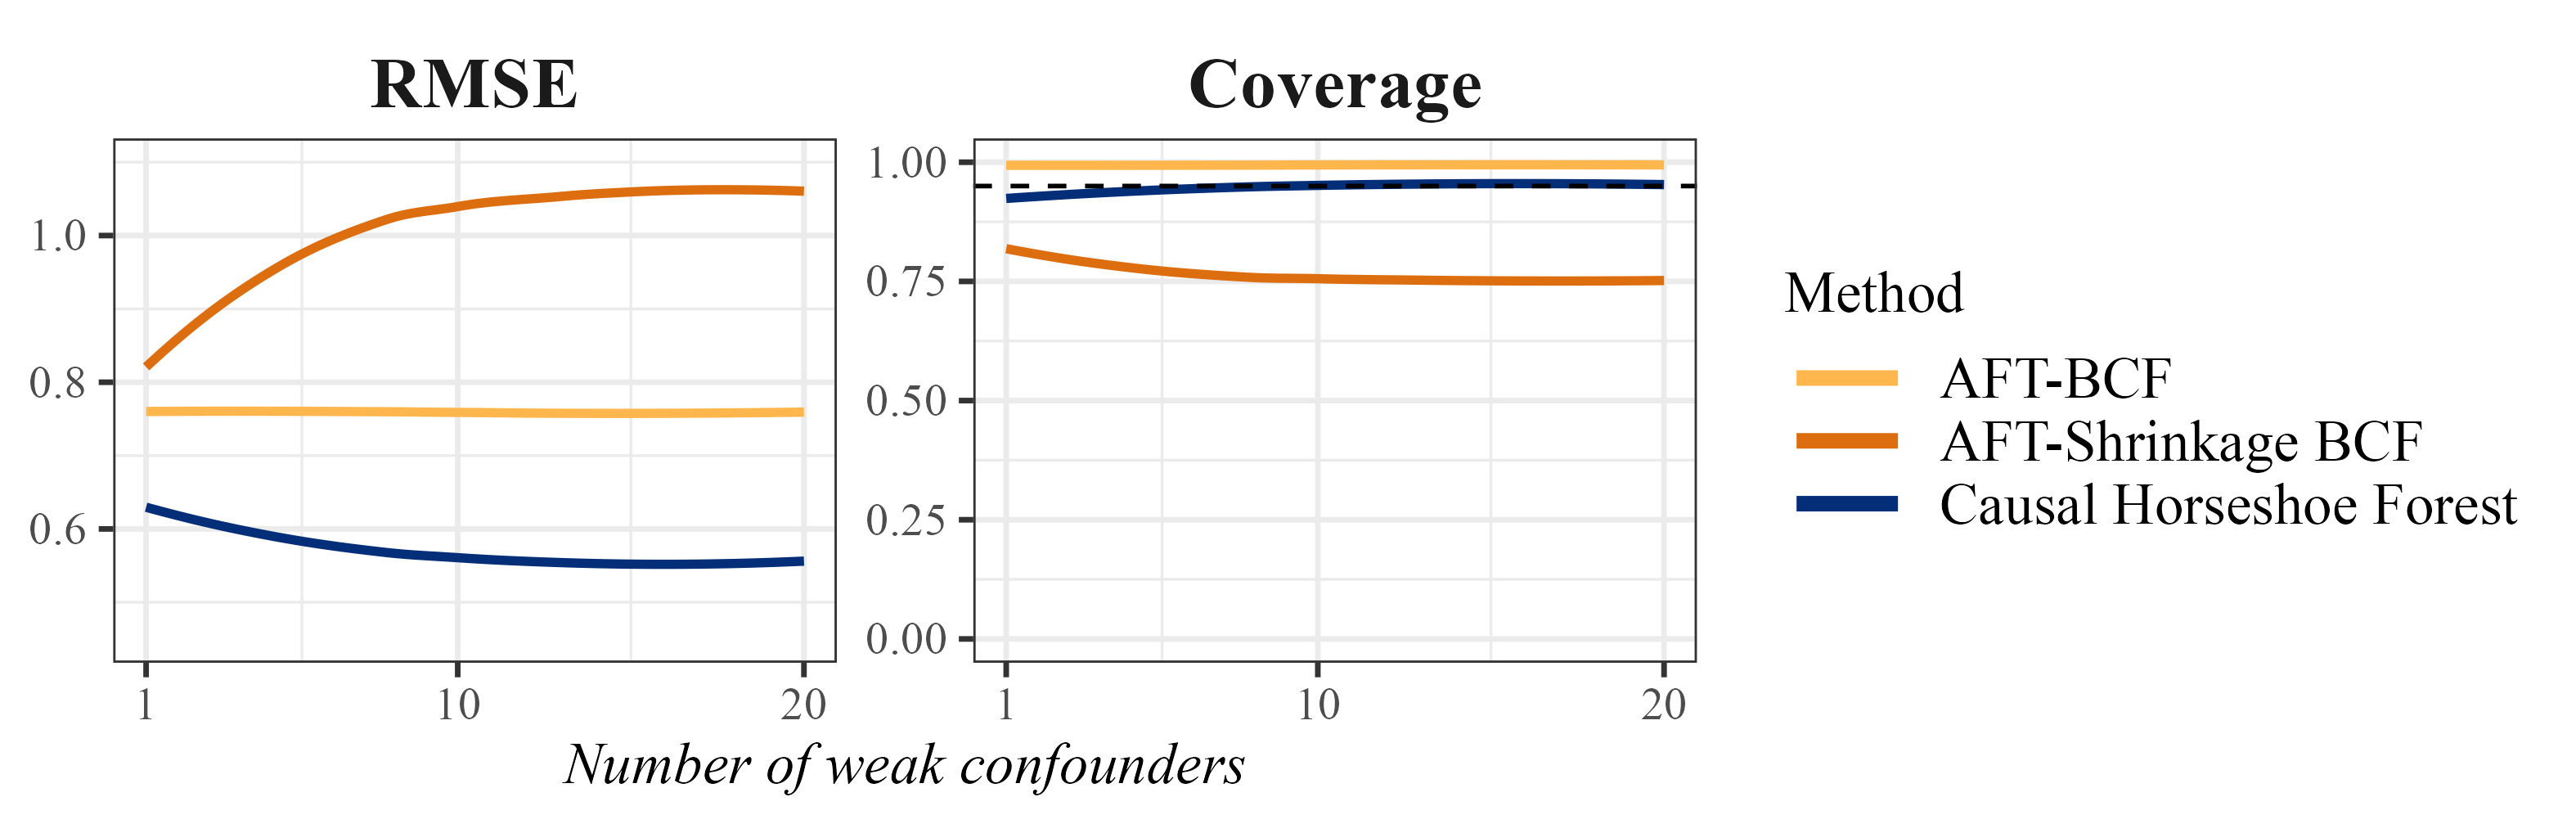
\includegraphics[width=\linewidth]{revision_ric.png}
    \caption{Regularisation-induced confounding simulation results. The figure shows RMSE (left) and empirical coverage (right) for heterogeneous treatment effect estimation as a function of the number of weak confounders. The dashed line indicates the nominal 95\% coverage level.}
      \captionsetup{font={color=Black}}
    \label{fig:ric}
\end{figure}


Continuous shrinkage on step heights provides the most stable form of regularisation for heterogeneous treatment effect estimation under different levels of weak confounding. 
Figure~\ref{fig:ric} reports RMSE and empirical coverage as functions of the number of weak confounders for the three methods considered. 
The Causal Horseshoe Forest maintains stable RMSE and near-nominal coverage as the number of weak confounders increases.
This behaviour reflects the ability of continuous shrinkage to preserve small but relevant signals and to provide well-calibrated uncertainty in high-dimensional settings.
AFT-BCF also exhibits largely constant RMSE as weak confounders are added, but coverage remains close to one across all settings. 
This suggests that regularisation through adjustment of the tree-structure priors is too weak in high-dimensional settings and results in overly wide posterior intervals.
AFT-Shrinkage BCF shows a sharp and monotone increase in RMSE as weak confounders are added, accompanied by a pronounced decline in coverage. 
The results suggest that aggressive sparsity induced by Dirichlet priors on covariate selection probabilities may exclude weak confounders, which is associated with higher bias and lower coverage under increasing regularisation-induced confounding.